% !TEX root = ../../RacefixThesis.tex
\graphicspath{{content/lcd/figures/}}

\mychapter{Determining loop carried dependencies}{chap:lcd}
\epigraph{\textit{Experience is a hard teacher because she gives the test first,
the lesson afterwards.}} %
{---\textsc{Vernon Sanders Law}} 

In order to perform the privatization described in chapter~\ref{chap:analysis}
the following precondition has to be met: the data is not involved in a
particular type of data-race that we call a \lcd.
That is, the fields must not be used as temporary storage between the
iterations of the loop (see listing~\ref{code:lcd-example-simple}). If we would
invert lines 4 and 6 then we would not be dealing with a \lcd. Reliably
determining whether or not a data-race is a \slcd has proven to be the most
challenging task in building this tool. 

To the best of the author's knowledge, at the time of implementation, there was
no algorithm for verifying the above mentioned precondition. Thus we we had to
go through several failed attempts (which are described in
section~\ref{sec:failed-attempts}) until we found the final solution that is
presented in section~\ref{sec:ifds-solution}.

\begin{lstlisting}[caption={Simple example of a loop carried dependency}, label
= {code:lcd-example-simple}]
//method called during the iterations of a loop
public void parallelContext() {
	//notice how the field 'lcd' is first read
    int temp = this.lcd;
    //...
    this.lcd = 42;
    //...
  }
\end{lstlisting}

\mysection{Definition of a \lcd}{def:lcd}
First, we represent a data-race on an object as follows:
\begin{itemize}
  \item a set of read accesses, \begin{math} R \end{math}
  \item a set of write accesses, \begin{math} W \end{math}
\end{itemize}

Second, a data-race is \emph{\textbf{not}} a \slcd if:

\textbf{\begin{math} \forall r\in R \end{math} is preceded on all possible
execution paths within by at least one \begin{math}w\in W\end{math}}

It is easier to comprehend the solutions we developed if you think in
terms of what is not an \slcd.


\mysection{Important cases of \lcds }{sec:lcd-examples}
In this section I expose a few cases of \slcds and explain how they are relevant
to describing the properties of a desired algorithm.

\begin{lstlisting}[caption={Branching instruction with a write on only one
path, this is an LCD}, label = {code:lcd-branch-write-on-one}]
public void branchingWriteOnlyOnePath() {
	if (this.condition)
      //something that isn't a write to the LCD field
    else
      this.LCD = 7;
    
    this.temp = this.LCD
}
\end{lstlisting}

\begin{lstlisting}[caption={Branching instruction with write on both paths,
this not an LCD}, label = {code:lcd-branch-write-on-both}]
public void branchingWriteOnBothPaths() {
    if (this.condition)
      this.notLCD = 42
    else
      this.notLCD = 6 * 9;
    this.temp = this.notLCD
}
\end{lstlisting}

The two examples from above show why it is imperative for every write
instruction to be covered on all paths by a write. Given
listing~\ref{code:lcd-branch-write-on-one} and the known limitations of static
analysis~\ref{th:static-analysis} (i.e. not being able to safely determine which
path is the one taken during runtime) we have to be conservative in our
assessment. Because one false negative will cause our transformations to change
a severe bug. Not being able to determine the actual execution path usually
means that our detection algorithm would provide false-positives; but, we also
have to consider that our tool is employed in the context of parallelizable
loops with tens, hundreds of thousands of iterations and that it is enough for a
branch to be executed only once to be a valid \lcd.

\begin{lstlisting}[caption={Multiple method calls, not an LCD}, label = {code:lcd-multiple-call-site}]
public void parallelContext() {
    this.bar();
    this.notLCD = 42;
    this.bar();
    this.temp = this.notLCD;
}
\end{lstlisting}

Listing~\ref{code:lcd-multiple-call-site} shows a case where an algorithm would
not work on graphs with no context sensitivity. Whenever the programmer would
want to traverse the whole call stack, method invocations would point to a new
CGNode~\ref{th:cgnode} with it's own control-flow graph. In our example at line
2 we start traversing the control flow graph of \emph{bar()}. When we have
finished the traversal of that node we'd have to continue though line 3 in
order to ensure correctness. Without any kind of context sensitivity this would
not be possible. Now, context sensitivity can be attained either by building it
directly into the graph (but this would lead to needlessly large graphs) or by
keeping a method call stack during the traversal. The IFDS algorithm uses the
latter.

\mysection{Failed Attempts}{sec:failed-attempts}
Our initial implementations, although not precise enough helped us identify
theoretical issues and increase the amount of our test data.

\mysubsection{Statement Ordering}{ssec:statement-ordering-approach}
Our first algorithm worked as described by the pseudo-code presented bellow. The
basic idea was that for all reads there has to be at least one write that
happens before it.

\begin{algorithm}[h]
\caption{determining loop carried dependencies based on statement ordering}
\begin{algorithmic}[1]
	\State $field$
	\State $R$ $\leftarrow$ ${\color{red} setOfReads(field)}$
	\State $W$ $\leftarrow$ ${\color{red} setOfWrites(field)}$
	\For{$read \in R$}
		\State $isNotLoopCarryDependency$ $\leftarrow$ false
		\For{$write \in W$}
			%${{\color{red} happensBefore}(write, read)}$
			\If{${{\color{red} happensBefore}(write, read)}$ }
				\State $isNotLoopCarryDependency$ $\leftarrow$ true
				\State break
			\EndIf
		\EndFor
	\State return $isNotLoopCarryDependency$
	\EndFor
\end{algorithmic}
\label{alg:LCD}
\end{algorithm}

The main issue here was the way this \emph{happens before} relation was
determined. We implemented a recursive algorithm that would start from the read
instructions and go backwards through the control-flow graph up until it exited
the parallel context or until it found a write instruction. If one read wasn't
preceded by a write then the corresponding data-race would be marked as a \lcd.
At first, we did not account for multiple execution paths (see
listings~\ref{code:lcd-branch-write-on-one} and
~\ref{code:lcd-branch-write-on-both}). As soon as we became aware of the problem
we tried fixing our algorithm but the solution was cumbersome so we binned it.

\mysubsection{Dominator approach}{ssec:dominator-approach}
This approach solved the problem that the algorithm presented
in~\ref{ssec:statement-ordering-approach} had by using an algorithm based on
dominators~\ref{th:dominators}. This time, instead of traversing the
control-flow graphs of each \emph{CGNodes} and make sure we link the nodes
together properly we use an interprocedural super-graph instead (a graph that
aggregates all the control-flow graphs of the CGNodes). Now that we have on
single graph describing the entire program we can easily establish the
domination (theory~\ref{th:dominators}) relation between instructions. Because
the definition of domination includes treating \emph{over-all possible paths}
cases, this dominator based approach solves the problems revealed by
example~\ref{code:lcd-branch-write-on-one}.

Our algorithm starts out by constructing the domination tree using WALA's
GenericDominator implementation which takes as an input an interprocedural
super-graph and a basic block denoting the entry point from which the tree is
constructed (in our case this block represents the start of the parallel
context).

After building the domination tree we try to verify the definition of a
\slcd~\ref{def:lcd}, by making sure that each read in R is dominated by the set
of writes W (this is a loose use of the phrase ``dominated by a set'', it can
just as easily be stated as being dominated by at least one write from the set
W).

Given the fact that the domination tree is built on a context
insensitive super-graph this approach has the handicap of not being able to
handle cases of the sort exemplified in listing
~\ref{code:lcd-multiple-call-site}. But it made us realize that the last piece
of the puzzle was infinite context sensitivity, which led us to the final
solution presented in the next section.

\mysection{IFDS Solution}{sec:ifds-solution}

This is a sound solution to the \slcd detection problem. It has none of the
disadvantages of the previous two attempts. It took us a while to notice that
our problem is in fact an \emph{Interprocedural, Finite, Distributive, subset
problems}~\ref{th:ifds}. But this realization opens the door to a very brief and
elegant solution.

Basically, we employ the standard IFDS algorithm with the following
particularities:
\begin{enumerate}

\item all data-races are evaluated in the same traversal, each pair of sets
\begin{math}(R,W)\end{math} being identified by an associated unique integer
number representing a \emph{data-flow fact}.

\item each set of reads \begin{math}R\end{math} is treated as a fact
(regardless which instruction from the same given set is encountered it is considered to be the
same fact). Each write from the set of writes \emph{W} kills the fact associated
with the corresponding pair \emph{R} set. 

\item we do backwards analysis (i.e. all edges of the super graph are inverted).
This choice has been made out of engineering and aesthetic concerns rather than
theoretical ones; backwards analysis gives us a direct answer to the question
``is this data-race a \lcd?''rather than ``is this data-race not a \lcd?''.

\item  At merging points we use the standard set reunion operator to determine
the facts that will be propagated; thus we propagate the fact corresponding to
our read.
\end{enumerate}

\begin{lstlisting}[caption={Code after which the graph in the example of an LCD
is made}, label={code:lcd-ifds-example-lcd}]
public void foo(){
	if(this.condition)
		bar();
	else
		this.lcd = 42;
	this.temp = this.lcd;
}
\end{lstlisting}

A graphical representation of how our algorithm works for the case illustrated
in listing~\ref{code:lcd-ifds-example-lcd} and can be seen in
Figure~\ref{fig:lcd-lcd}; a step-by-step explanation follows:

\begin{figure}
        \begin{subfigure}[h]{0.3\textwidth}
                \centering
                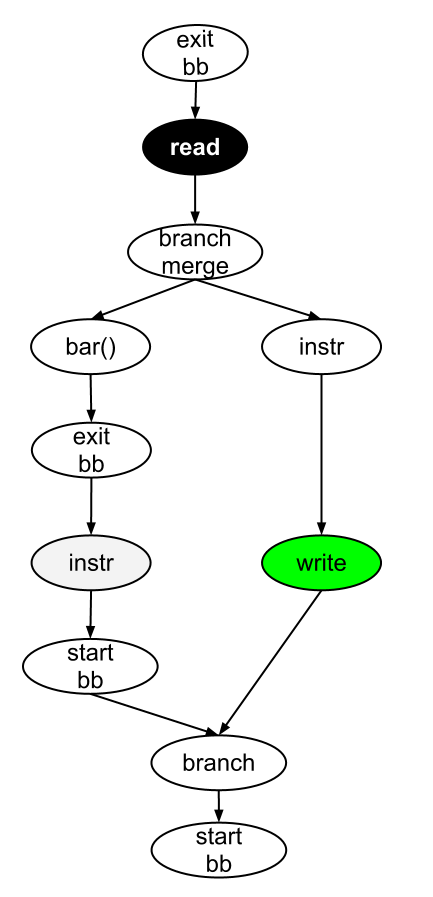
\includegraphics[width=\textwidth]{lcd01}
                \caption{}
                \label{fig:lcd-lcd01}
        \end{subfigure}%
        \begin{subfigure}[h]{0.3\textwidth}
                \centering
                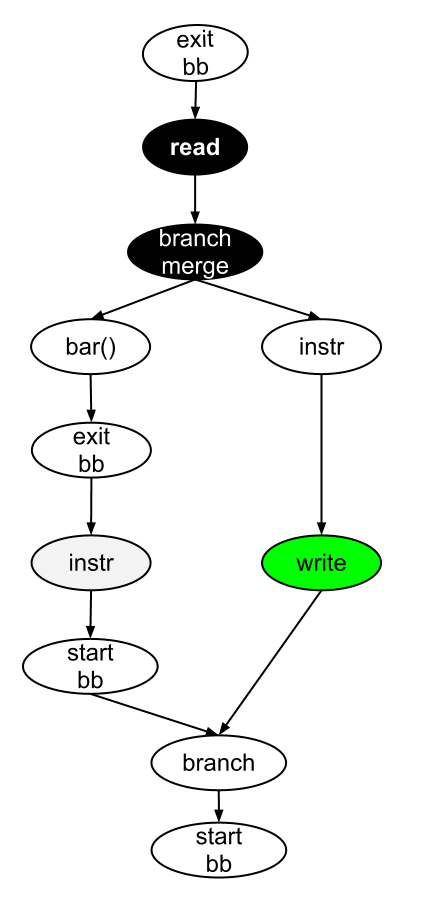
\includegraphics[width=\textwidth]{lcd02}
                \caption{}
                \label{fig:lcd-lcd02}
        \end{subfigure}
        \begin{subfigure}[h]{0.3\textwidth}
                \centering
                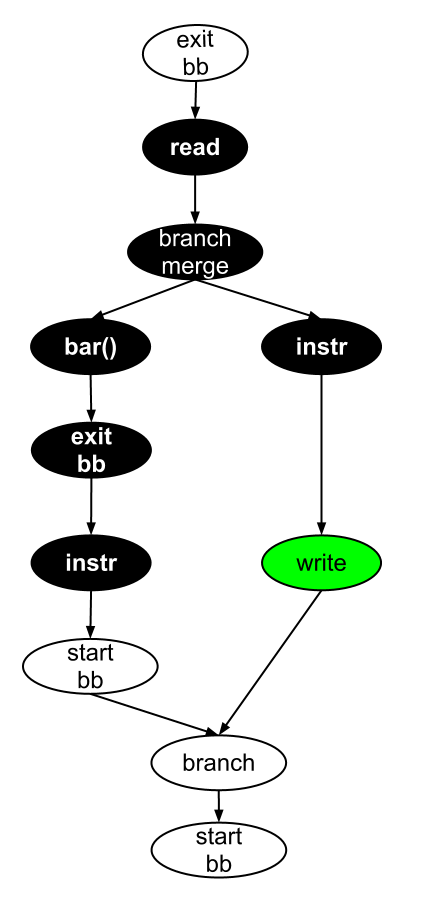
\includegraphics[width=\textwidth]{lcd03}
                \caption{}
                \label{fig:lcd-lcd03}
        \end{subfigure}
        
        \begin{subfigure}[h]{0.3\textwidth}
                \centering
                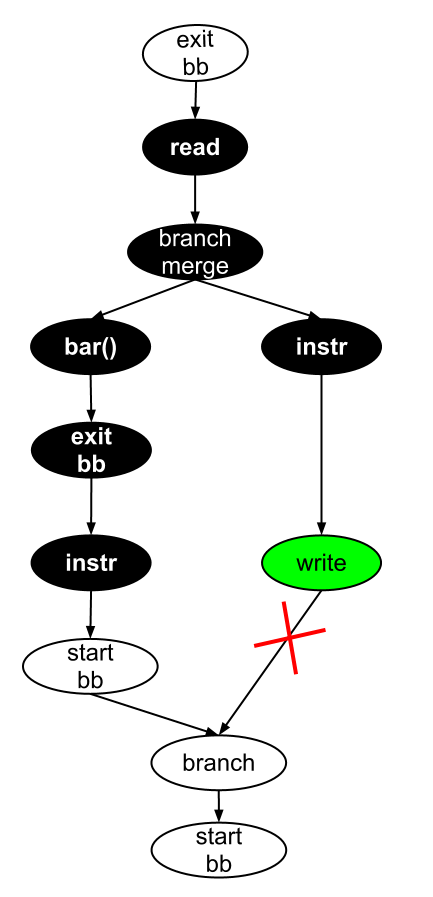
\includegraphics[width=\textwidth]{lcd04}
                \caption{}
                \label{fig:lcd-lcd04}
        \end{subfigure}
        \begin{subfigure}[h]{0.3\textwidth}
                \centering
                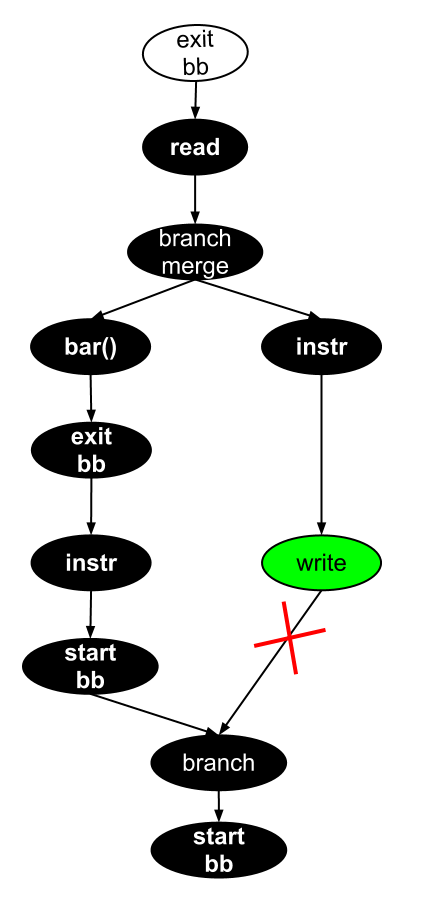
\includegraphics[width=\textwidth]{lcd05}
                \caption{}
                \label{fig:lcd-lcd05}
        \end{subfigure}
        \caption{A graphical representation of how our
        algorithm treats the case of an LCD on a branch}\label{fig:lcd-lcd}
\end{figure}

\begin{enumerate}
  \item [a)] we encountered a read, so from now on we propagate the fact
  corresponding to that set of reads (in this particular case, the set contains
  only one read).
  \item [b)] when a node has more children (i.e it is the onset of multiple
  execution paths) the preexisting facts are simply propagated on both.
  \item [c)] on the left path, a method invocation is encountered. The
  propagation of facts is unaffected by method calls.
  \item [d)] on the right path, we've encountered a write access from the set
  corresponding to one our known facts, we kill said fact (i.e. we no longer
  propagate it to the next instruction)
  \item[e)] even though the fact on the right path was killed, the one on the
  left could propagate unhindered. Now, at the initial branching point we have
  two paths: one with a set of one fact, one with an empty set. At merging
  points we use the standard set reunion operator to determine the facts that
  will be propagated; thus we propagate the fact corresponding to our read.
  We've reached the end of the scope of our analysis with one fact live,
  this means that the corresponding data race is labeled as a \lcd.
\end{enumerate}

The second example will treat the case of a write on both branches, it is
represented by listing~\ref{code:lcd-ifds-example-notlcd} and
Figure~\ref{fig:lcd-notlcd}

\begin{lstlisting}[caption={Code after which the graph in the example of an LCD
is made}, label={code:lcd-ifds-example-notlcd}]
public void foo(){
	if(this.condition)
		bar(); 
	else 
		this.lcd = 42;
	this.temp = this.lcd;
}
public void bar(){
	this.lcd = 6 * 9;
}
\end{lstlisting}
\begin{enumerate}
  \item [a), b)] same as in Figure~\ref{fig:lcd-lcd}
  \item [c)] we have encountered writes on both execution paths and the method
  invocation on the left side doesn't affect the outcome at all.
  \item [d)] the facts on both execution paths are killed so no facts propagate
  to the top, meaning we have no \lcds.
\end{enumerate}

\begin{figure}
        \begin{subfigure}[l]{0.3\textwidth}
                \centering
                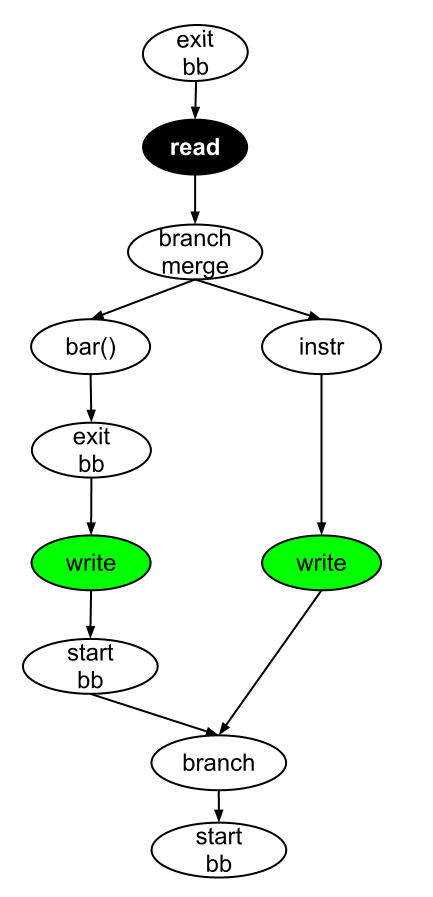
\includegraphics[width=\textwidth]{nonlcd01}
                \caption{}
                \label{fig:lcd-notlcd01}
        \end{subfigure}%
        \begin{subfigure}[r]{0.3\textwidth}
                \centering
                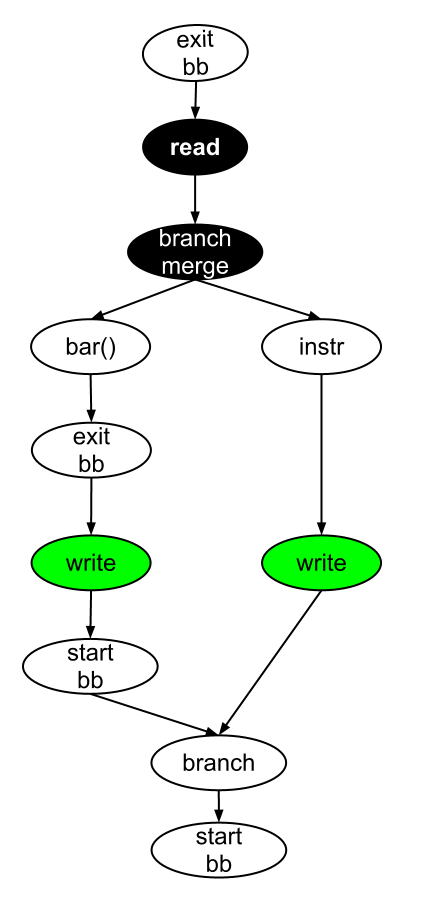
\includegraphics[width=\textwidth]{nonlcd02}
                \caption{}
                \label{fig:lcd-notlcd02}
        \end{subfigure}
        
        \begin{subfigure}[l]{0.3\textwidth}
                \centering
                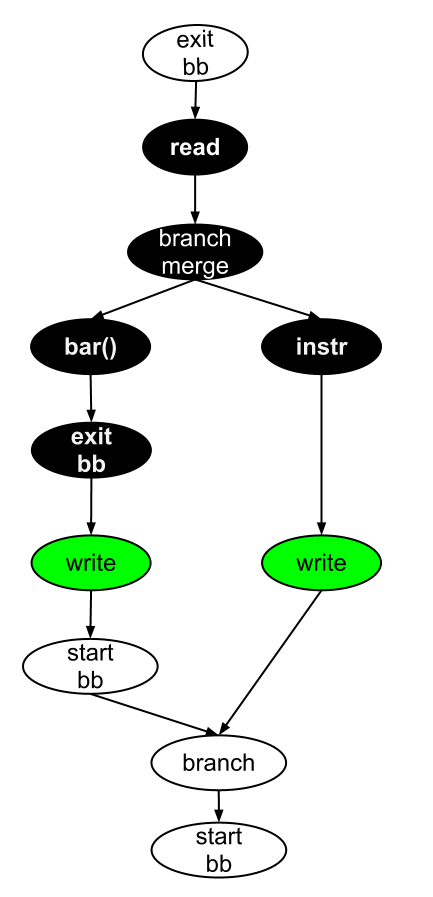
\includegraphics[width=\textwidth]{nonlcd03}
                \caption{}
                \label{fig:lcd-notlcd03}
        \end{subfigure}
            \begin{subfigure}[r]{0.3\textwidth}
                \centering
                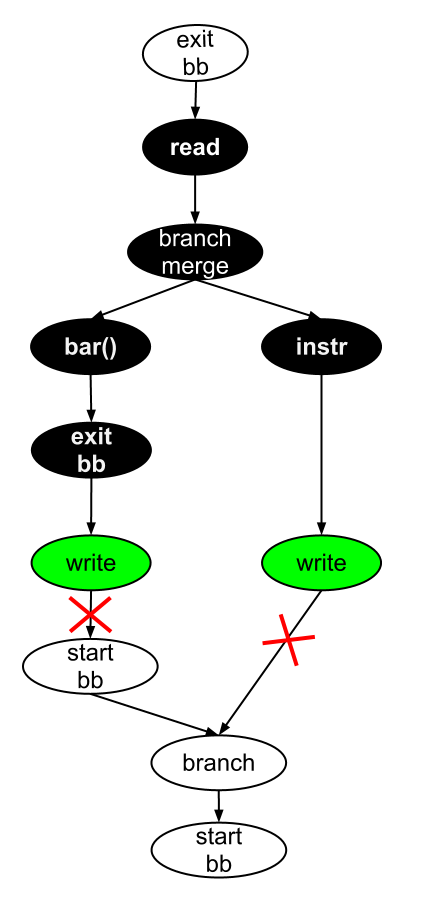
\includegraphics[width=\textwidth]{nonlcd04}
                \caption{}
                \label{fig:lcd-notlcd04}
        \end{subfigure}
        \caption{The case in which we don't have an LCD}\label{fig:lcd-notlcd}
\end{figure}

\mysubsection{Evaluation}{ssec:lcd-evaluation}
Our algorithm has been tested on Jmol~\cite{Jmol-site} and out of a total of
\textbf{163} data-races \textbf{63} are labeled as \lcds. After manual
inspection of each of the supposed \slcds, we have determined that the property
indeed holds true for them. This gives us solid empirical evidence of the
soundness of our analysis.
